\documentclass{beamer}
\usetheme{metropolis}
\usepackage{graphicx}
\usepackage{amsmath}
\usepackage{url}

\def\rcurs{{\mbox{$\resizebox{.16in}{.08in}{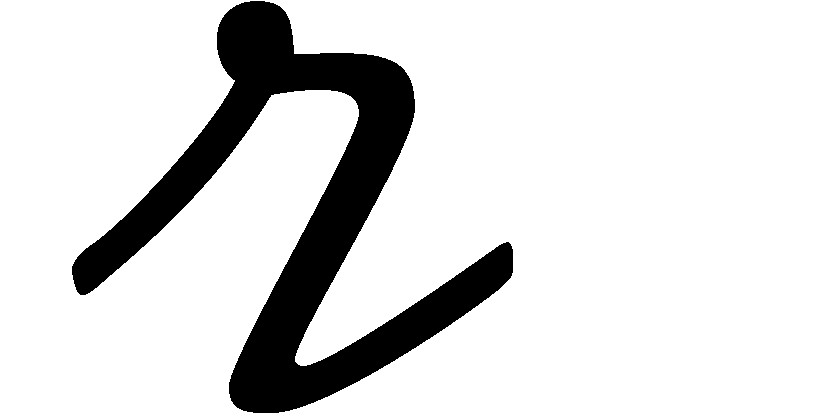
\includegraphics{ScriptR}}$}}}
\def\brcurs{{\mbox{$\resizebox{.16in}{.08in}{
\includegraphics{BoldR}}$}}}
\def\hrcurs{{\mbox{$\hat \brcurs$}}}

\title{Electromagnetc Theory: PHYS330}
\author{Jordan Hanson}
\institute{Whittier College Department of Physics and Astronomy}

\begin{document}
\maketitle

\section{Summary}

\begin{frame}{Week 5 Summary}
\begin{enumerate}
\item Current density and continuity equation
\item The divergence and curl of $\vec{B}$-fields
\item The magnetic vector potential, $\vec{B} = \nabla \times \vec{A}$
\begin{itemize}
\item Vector calculus theorems
\item Boundary conditions
\item Multipole expansion
\end{itemize}
\item Magnetic fields in matter
\begin{itemize}
\item Magnetization
\item Field of a magnetized object
\item The auxiliary field, $\vec{H}$
\item Linear magnetic media
\end{itemize}
\end{enumerate}
\end{frame}

\section{Current density and continuity equation}

\begin{frame}{Current density and continuity equation}
Let the \textit{current density} $\vec{J}$ be defined by
\begin{equation}
\vec{J} = \rho \vec{v}
\end{equation}
Units: current per unit area (other definitions available for different geometries).  So it's reasonable to obtain the whole scalar current by integrating:
\begin{equation}
I = \int_{\mathcal{S}} \vec{J} \cdot d\vec{a}
\end{equation}
If we want to account for the charge leaving a volume $\mathcal{V}$ through a closed surface $\mathcal{S}$ is
\begin{align}
\oint_{\mathcal{S}} \vec{J} \cdot d\vec{a} &= \int_{\mathcal{V}} (\nabla \cdot \vec{J}) d\tau \\
\int_{\mathcal{V}} (\nabla \cdot \vec{J}) d\tau &= -\frac{d}{dt} \int_{\mathcal{V}} \rho d\tau = -\int_{\mathcal{V}} \frac{\partial \rho}{\partial t} d\tau
\end{align}
\end{frame}

\begin{frame}{Current density and continuity equation}
This is true for \textit{any} volume, so the integrands must be equal:
\begin{equation}
\nabla \cdot \vec{J} = -\frac{\partial \rho}{\partial t}
\end{equation}
This is called the continuity equation, and it also arises in quantum mechanics.  If $\partial\rho/\partial t = 0$, then we have a \textbf{steady current.} \\ \vspace{0.5cm}
Suppose we have a current density $\vec{J}(\vec{r}) = I_0(t) \hat{r}/r^2$, with $I_0(t) = \delta(t-t_0)$.  Find $\rho(t)$, the charge density as a function of time in the region containing $\vec{J}$. (Breakout rooms).
\end{frame}

\section{The Divergence of $B$-fields}

\begin{frame}{The Divergence of $B$-fields}
The Biot-Savart law states that
\begin{equation}
\vec{B}(\vec{r}) = \frac{\mu_0}{4\pi} \int \frac{\vec{J}(\vec{r'}) \times \hrcurs }{\rcurs} d\tau'
\end{equation}
\begin{figure}
\centering
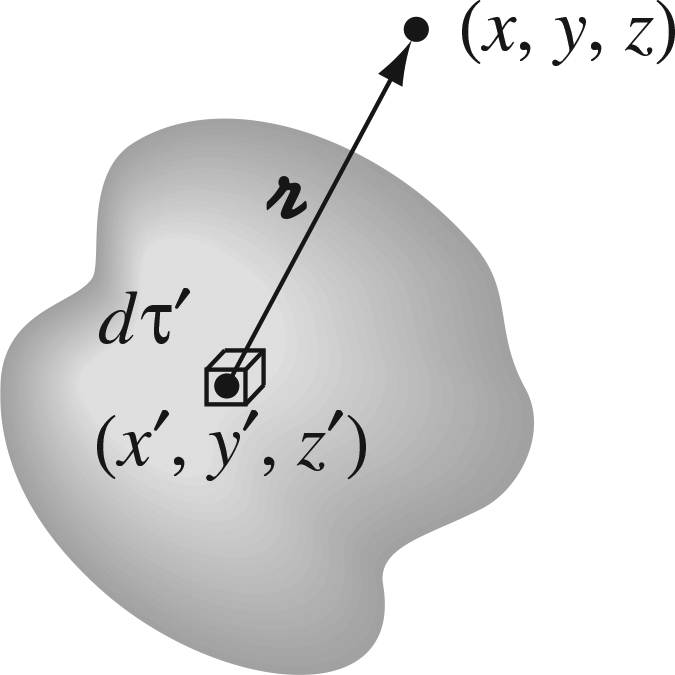
\includegraphics[width=3cm]{figures/5_30.png}
\caption{\label{fig:biot} Definitions of coordinates in variables for derivation of divergence of B-fields.  The gray region represents charges and current densities.}
\end{figure}
\end{frame}

\begin{frame}{The Divergence of $B$-fields}
Take the divergence of the Biot-Savart law, but then use a product rule for the integrand.
\begin{align}
\nabla \cdot \vec{B} =& \frac{\mu_0}{4\pi} \int \nabla \cdot \left( \vec{J} \times \frac{\hrcurs}{\rcurs^2}\right) d\tau' \\
\nabla \cdot \left( \vec{J} \times \frac{\hrcurs}{\rcurs^2}\right) &= \frac{\hrcurs}{\rcurs^2} \cdot (\nabla \times \vec{J}) - \vec{J} \cdot \left( \nabla \times \frac{\hrcurs}{\rcurs^2} \right)
\end{align}
\begin{itemize}
\item $\nabla \times \vec{J} = 0$, because this is like taking $df(x)/dx'$.
\item We showed in Chapter 1 that $\nabla \times \frac{\hrcurs}{\rcurs^2} = 0$.  Is this visually obvious?
\end{itemize}
Thus,
\begin{equation}
\boxed{
\nabla \cdot \vec{B} = 0
}
\end{equation}
\end{frame}

\begin{frame}{The Divergence of $B$-fields}
From warmup exercises, we know that we can therefore write
\begin{equation}
\vec{B} = \nabla \times \vec{A}
\end{equation}
(Breakout rooms): create three divergence-less vector fields.  One in Cartesian coordinates, one in cylindrical coodinates, and one in spherical.  Exclude trivial cases like $\vec{B} = 0$.
\end{frame}

\section{Conclusion}

\begin{frame}{Week 5 Summary}
\begin{enumerate}
\item Current density and continuity equation
\item The divergence and curl of $\vec{B}$-fields
\item The magnetic vector potential, $\vec{B} = \nabla \times \vec{A}$
\begin{itemize}
\item Vector calculus theorems
\item Boundary conditions
\item Multipole expansion
\end{itemize}
\item Magnetic fields in matter
\begin{itemize}
\item Magnetization
\item Field of a magnetized object
\item The auxiliary field, $\vec{H}$
\item Linear magnetic media
\end{itemize}
\end{enumerate}
\end{frame}

\end{document}
